%! TEX root = main.tex

\subsection{Validation: 2D Cylinder, $Re=\num{40}$}\label{sec:val_2d_cylinder_re40}

We used the 2D cylinder flow at $Re=40$ for validation because it has a similar configuration with the $Re=200$ case.
The $Re=40$ flow, however, does not have vortex shedding and reaches a steady-state solution, making it easier to validate the temporal behaviors in the solvers.
Well-established experimental data exist for $Re=40$.

The computational domain is $[-10$, $30]$ $\times$ $[-10$, $10]$, and $t \in [0, 20]$.
A cylinder with a radius of $0.5$ sits at $x=y=0$.
Nondimensional density is $1$, and kinematic viscosity is $0.025$.
The initial conditions are $u=1$ and $v=0$.
The boundary conditions are $u=1$ and $v=0$ on $x=-10$, $y=-10$, and $y=10$.
At the outlet, $x=30$, the boundary conditions are 1D convective conditions:
\begin{equation}\label{eq:convec-bc}
    \left\{
    \begin{aligned}
        &\pdiff{u}{t} + c\pdiff{u}{\vec{n}} = 0 \\
        &\pdiff{v}{t} + c\pdiff{v}{\vec{n}} = 0 \\
    \end{aligned}
    \right.
\end{equation}
where $\vec{n}$ is the normal vector of the boundary (pointing outward), and $c$ is the convection speed.
In this work, we used $c=1$.

The PetIBM validation ran on a machine with an NVIDIA K40 GPU and 6 cores of Intel i7-5930K.
The grid resolution was $562 \times 447$ with $\Delta t=\num{1e-2}$.
The tolerance for all linear solvers in PetIBM was $\num{1e-14}$, and same configurations of the linear solvers were used as in the TGV simulations.
PetIBM used double-precision floats.

We used two different PINN solvers in this validation because both solvers would also be used later in the $Re=200$ case.
The first one is the unsteady PINN solver, which solves the unsteady Navier-Stokes equations as shown in figure \ref{fig:pinn-workflow}.
The second one is the steady PINN solver, which solves the steady Navier-Stokes equations.
The workflow of the steady PINN solver works similar to that in figure \ref{fig:pinn-workflow} except that all time-related terms and losses are dropped.

Both PINN solvers used \num{6} hidden layers and \num{512} neurons per layer in the MLP network.
The Adam optimizer had the same parameters as in the TGV case and ran for \num{400000} optimization iterations.
The learning rate scheduler was a cyclical learning rate with $\eta_{low}=\num{1e-6}$, $\eta_{high}=\num{1e-2}$, $N_c=\num{5000}$, and $\gamma={0.99998}$.
The hardware used was one NVIDIA A100 GPU for both PINN solvers.
Again, the PINN solvers used single-precision floats.

To evaluate PDE losses, \num{256000000} spatial-temporal points were randomly sampled from the computational domain and the desired simulation time range.
Each iteration, \num{25600} points were used to evaluate the PDE losses, so the Adam optimizer would see each points \num{40} times during the \num{400000}-iteration optimization.
\num{25600000} points were sampled on the boundaries at $y=\pm 10$, and \num{12800000} were sampled on the boundaries of $x=-10$ and $x=30$.
On the cylinder surface, the number of spatial-temporal points were \num{5120000}.
In each iteration, \num{2560}, \num{1280}, and \num{512} points were used, respectively.

Figure \ref{fig:cylinder-re40-pinn-loss} shows the training history of the PINN solvers.
The total loss of the steady PINN solver converged to around \num{e-4}, while that of the unsteady PINN solver converged to around \num{e-2} after about 26 hours of training.
Readers should be aware that the configuration of the PINN solvers might not be optimal, so the accuracy and the computational cost shown in this figure should not be treated as an indication of PINNs' general performance.
In our experience, it is possible to reduce the run time in half but obtain the same level of accuracy by adjusting the number of spatial-temporal points used per iteration.

\begin{figure}
    \centering%
    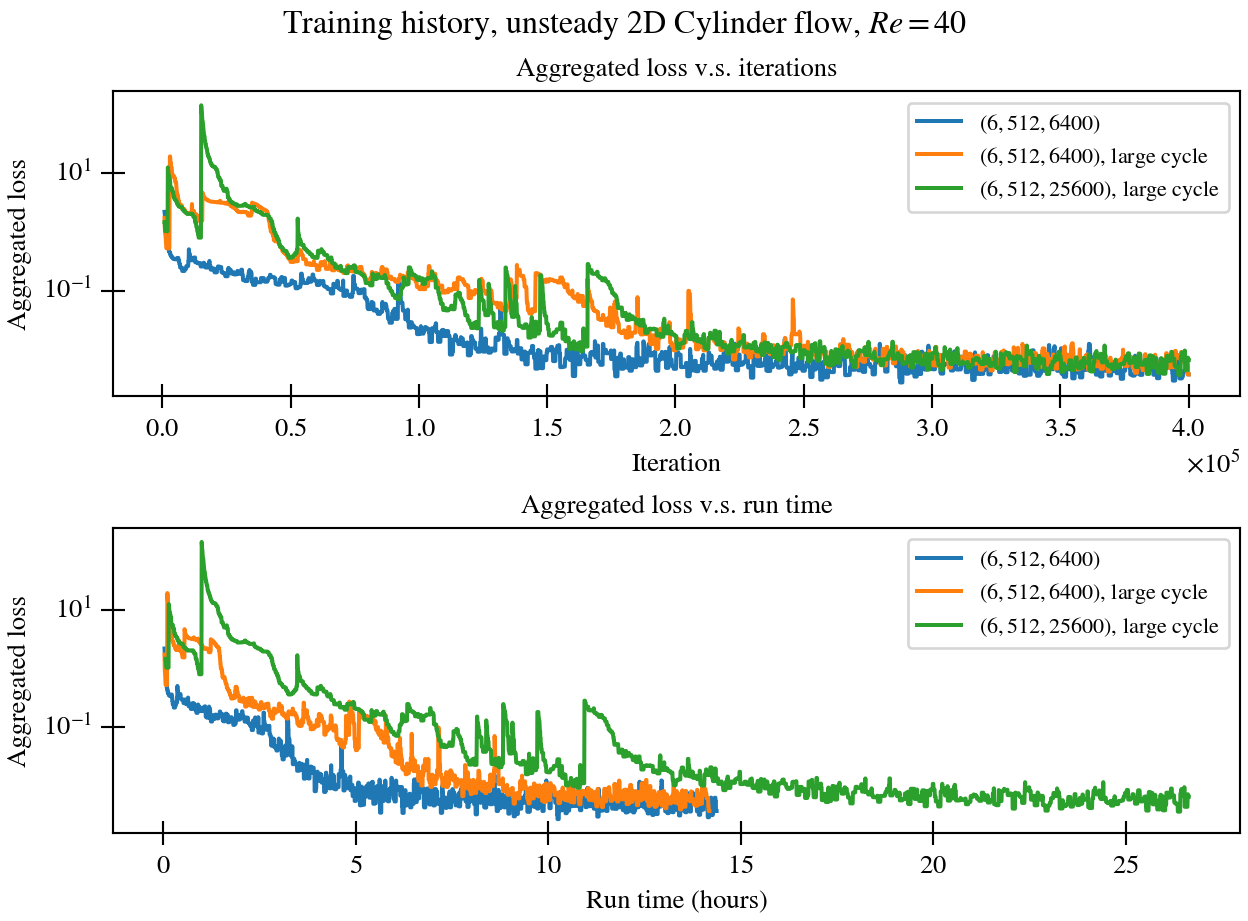
\includegraphics[width=\columnwidth]{cylinder-2d-re40/loss-hist-unsteady.png}%
    \caption{%
        Training convergence history of 2D cylinder flow at $Re=\num{40}$ for both steady and unsteady PINN solvers.
    }
    \label{fig:cylinder-re40-pinn-loss}%
\end{figure}

Figure \ref{fig:cylinder-re40-contours} shows the comparison of the steady-state flow fields (i.e., the snapshots at $t=20$ for PetIBM and the unsteady PINN solver).
The PINN solvers' results visually agree with PetIBM's.
The variation in the vorticity of PINNs only happens at the contour line of \num{0}, so it is likely caused by trivial rounding errors.
Note that vorticity is obtained by post-processing for all solvers.
PetIBM used central difference to calculate the vorticity, while the PINN solvers used automatic differentiation to obtain it.

Figure \ref{fig:cylinder-re40-drag-lift} gives the drag and lift coefficients ($C_D$ and $C_L$) with respect to simulation time.
Note the steady PINN solver's results were omitted as it does not have time history.
The PINN's results visually agrees with PetIBM's.
Table \ref{table:cylinder-re40-cd-comparison} compares the values of $C_D$ against the experimental data and simulation data from literature.
As seen from the table, values from different works in the literature do not closely agree with each other.
Though there is not a single value to compare against, at least the $C_D$ from the PINN solvers and PetIBM fall into the range of others' works.
We consider the results of $C_D$ validated for the PINN solvers and PetIBM.

\begin{figure}
    \centering%
    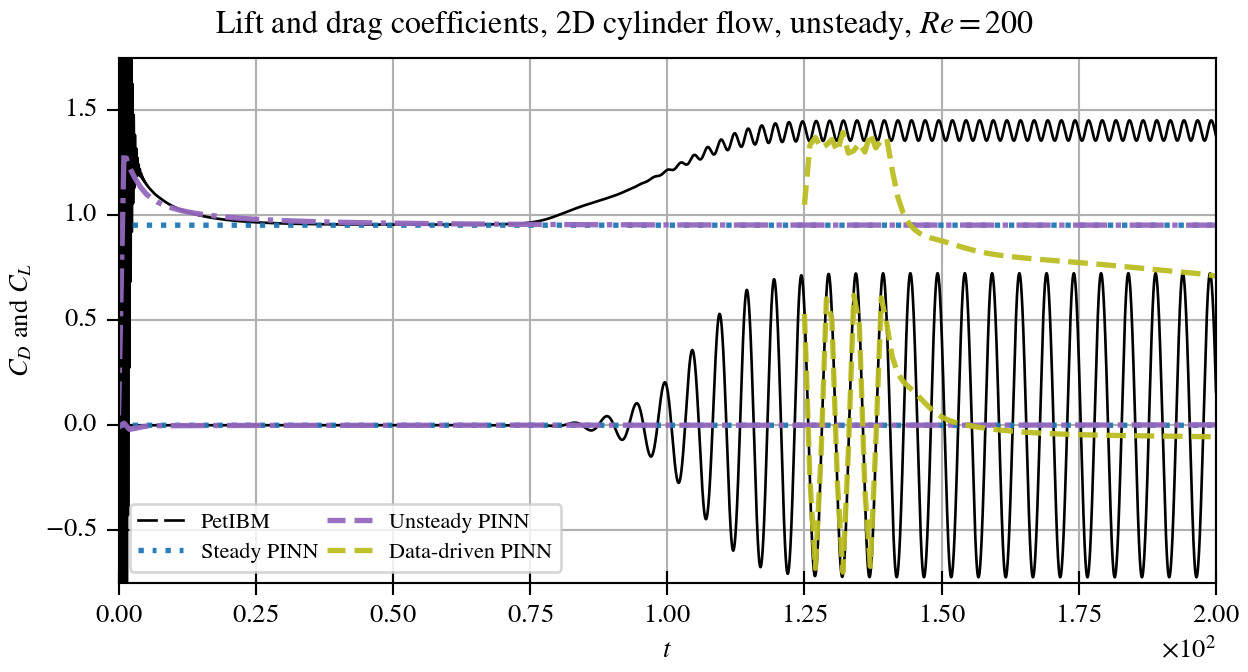
\includegraphics[width=\columnwidth]{cylinder-2d-re40/drag-lift-coeffs}%
    \caption{%
        Drag and lift coefficients of 2D cylinder flow at $Re=\num{40}$ w/ PINNs
    }
    \label{fig:cylinder-re40-drag-lift}%
\end{figure}

\begin{table}
    \centering%
    \begin{threeparttable}[b]
        \begin{tabular}{lccc}
            \toprule
            & $C_D$ & $C_{D_p}$ & $C_{D_f}$ \\
            \midrule
            Steady PINN &  &  &  \\
            Unsteady PINN & 1.60 & 1.06 & 0.55 \\
            PetIBM & 1.63 & 1.02 & 0.61 \\
            Rosetti et al., 2012\cite{rosetti_urans_2012}\tnote{1} & \num{1.74+-0.09} & n/a & n/a \\
            Rosetti et al., 2012\cite{rosetti_urans_2012}\tnote{2} & 1.61 & n/a & n/a \\
            Sen et al., 2009\cite{sen_steady_2009}\tnote{2} & 1.51 & n/a & n/a \\
            Park et al., 1988\cite{park_numerical_1998}\tnote{2} & 1.51 & 0.99 & 0.53 \\
            Tritton, 1959\cite{tritton_experiments_1959}\tnote{1} & 1.48--1.65 & n/a & n/a \\
            Grove et al., 1964\cite{grove_experimental_1964}\tnote{1} & n/a & 0.94 & n/a \\
            \bottomrule
        \end{tabular}%
        \begin{tablenotes}
            \footnotesize
            \item [1] Experimental result
            \item [2] Simulation result
        \end{tablenotes}
        \caption{%
            Validation of drag coefficients.%
            $C_D$, $C_{D_p}$, and $C_{D_f}$ denote the coefficients of total drag, pressure drag, %
            and friction drag, respectively.%
        }%
        \label{table:cylinder-re40-cd-comparison}
    \end{threeparttable}
\end{table}%

Finally, figure \ref{fig:cylinder-re40-pinn-surfp} shows the pressure distribution on the cylinder surface.
Again, though there is not a single solution that all works agree upon, the results from PetIBM and the PINN solvers visually agree with literature.
We considered PetIBM and both PINN solvers validated.

\begin{figure}
    \centering%
    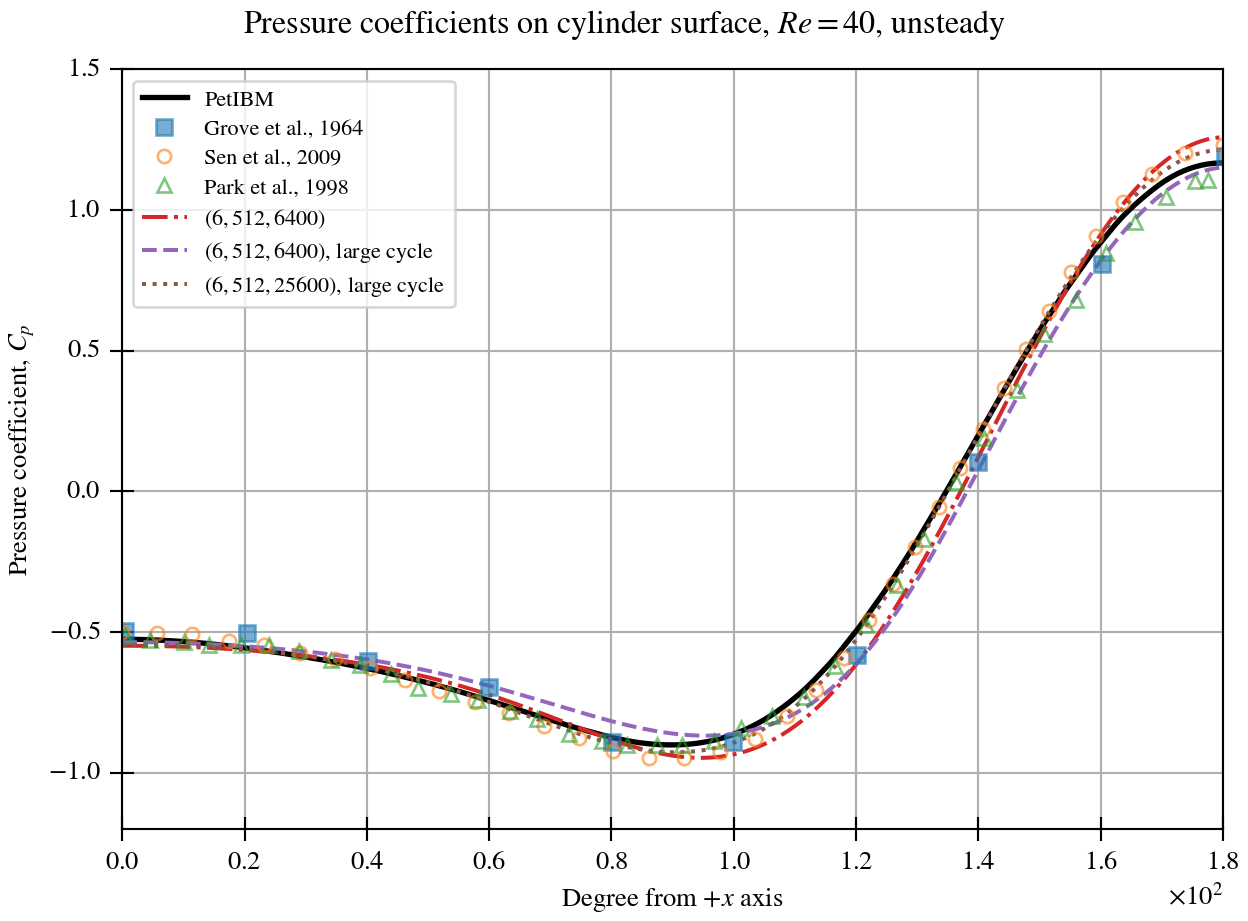
\includegraphics[width=0.95\columnwidth]{cylinder-2d-re40/surface-pressure-unsteady}%
    \caption{%
        Surface pressure distribution of 2D cylinder flow at $Re=\num{40}$ w/ unsteady PINN
    }
    \label{fig:cylinder-re40-pinn-surfp}%
\end{figure}

\begin{figure*}
    \centering%
    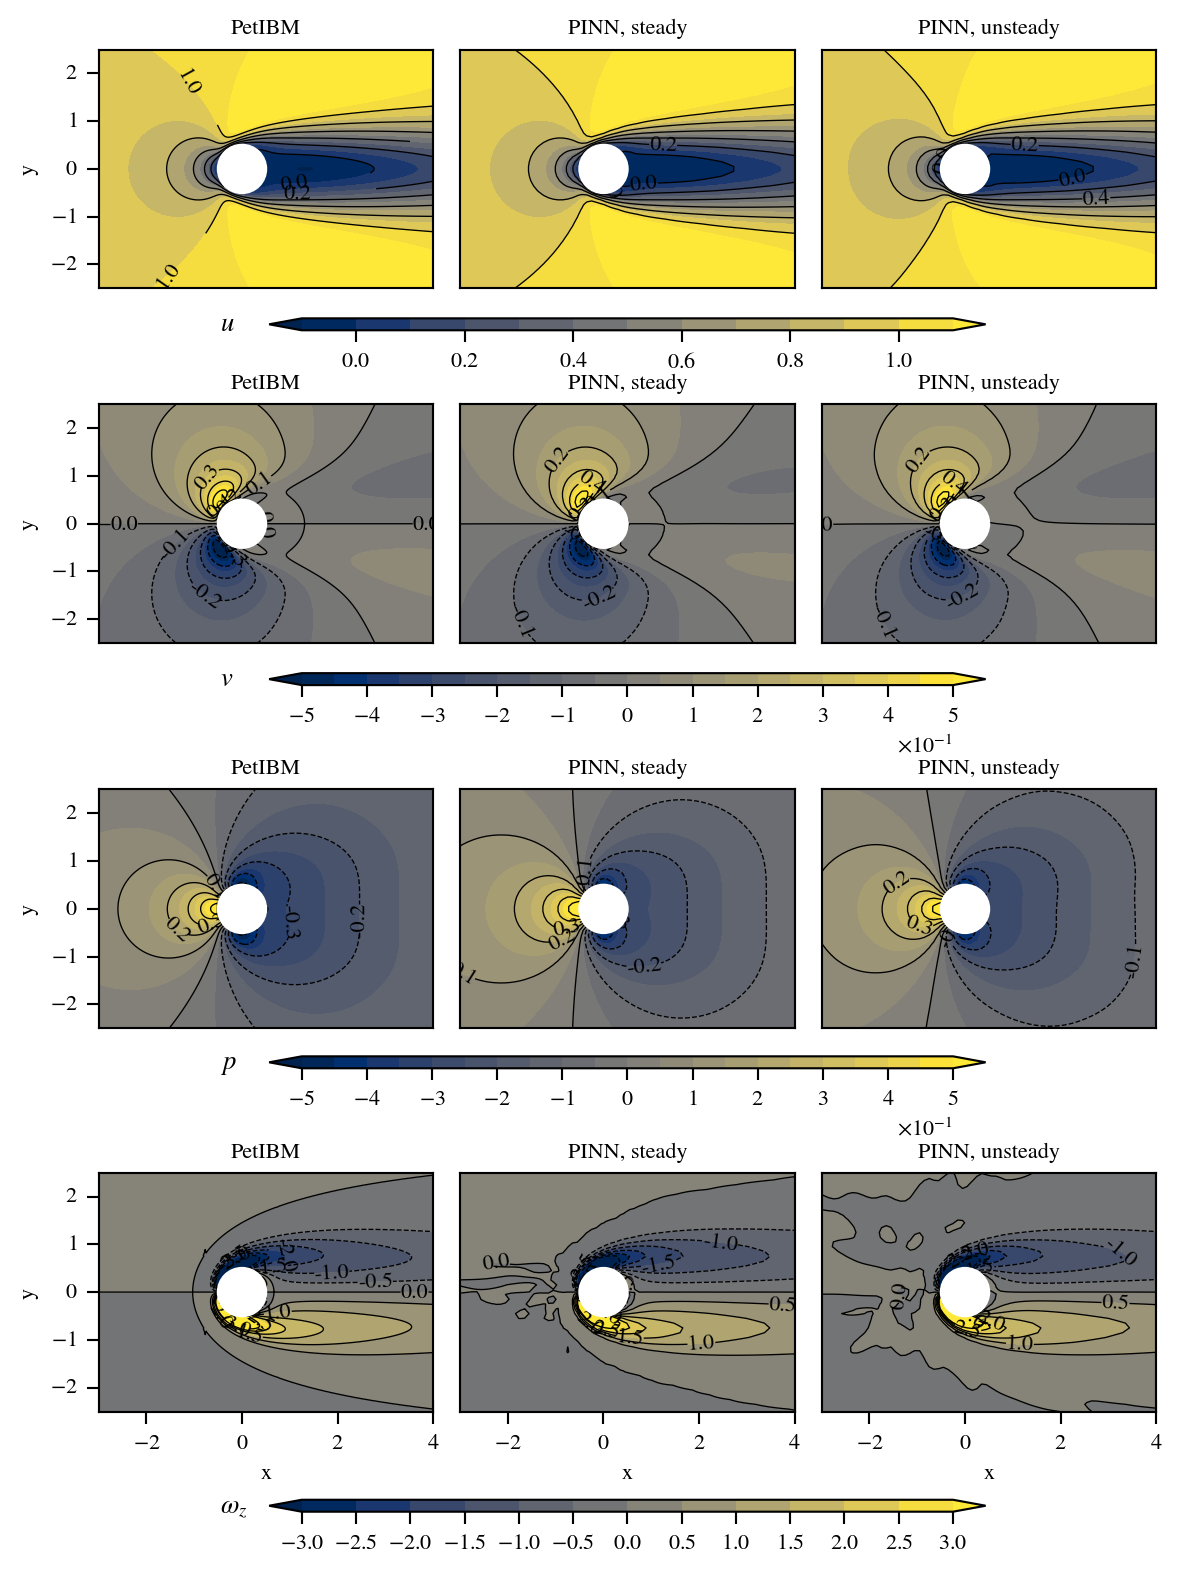
\includegraphics{cylinder-2d-re40/contour-comparison}%
    \caption{%
        Contour comparison of 2D cylinder flow at $Re=\num{40}$ w/ unsteady PINN
    }
    \label{fig:cylinder-re40-contours}%
\end{figure*}

% vim:ft=tex:
